\newpage
\vspace{6cm}
\section{RESULT}
\hspace{0.7cm}Firstly, we have to start the server so it can listen to the coming connections from clients:
\begin{figure}[h]
\centering
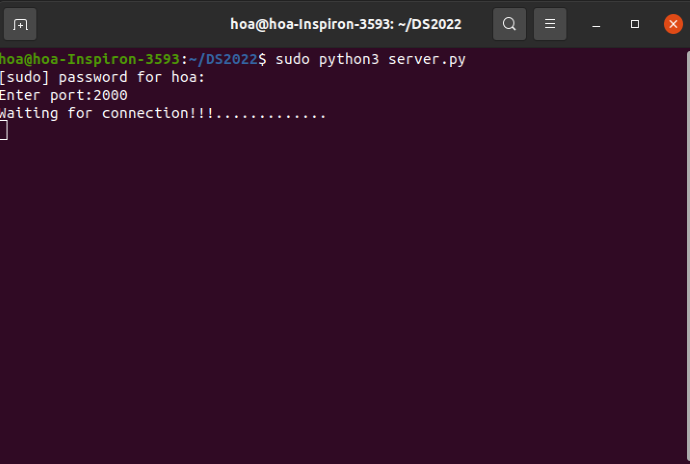
\includegraphics{images/result_1.png}
\end{figure}

\hspace{0.7cm}When the client side is started, the user needs to enter the port number. If the port number is different from that from the server side, the connection is denied:

\begin{figure}[h]
\centering
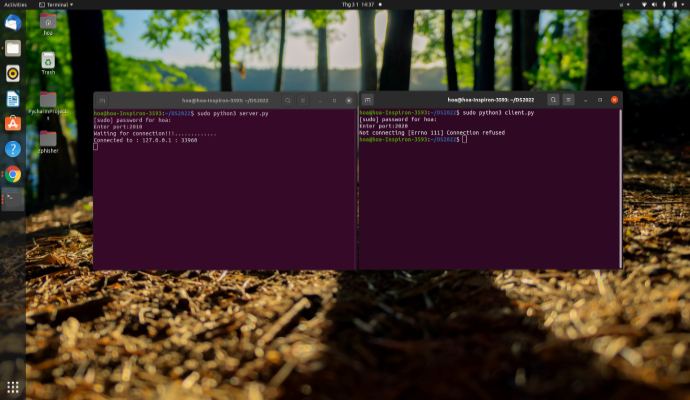
\includegraphics{images/result_2.png}
\end{figure}
\newpage
\hspace{0.7cm} In case the port number is the same, the connection is accepted. There can be multiple clients but only one server:

\begin{figure}[h]
\centering
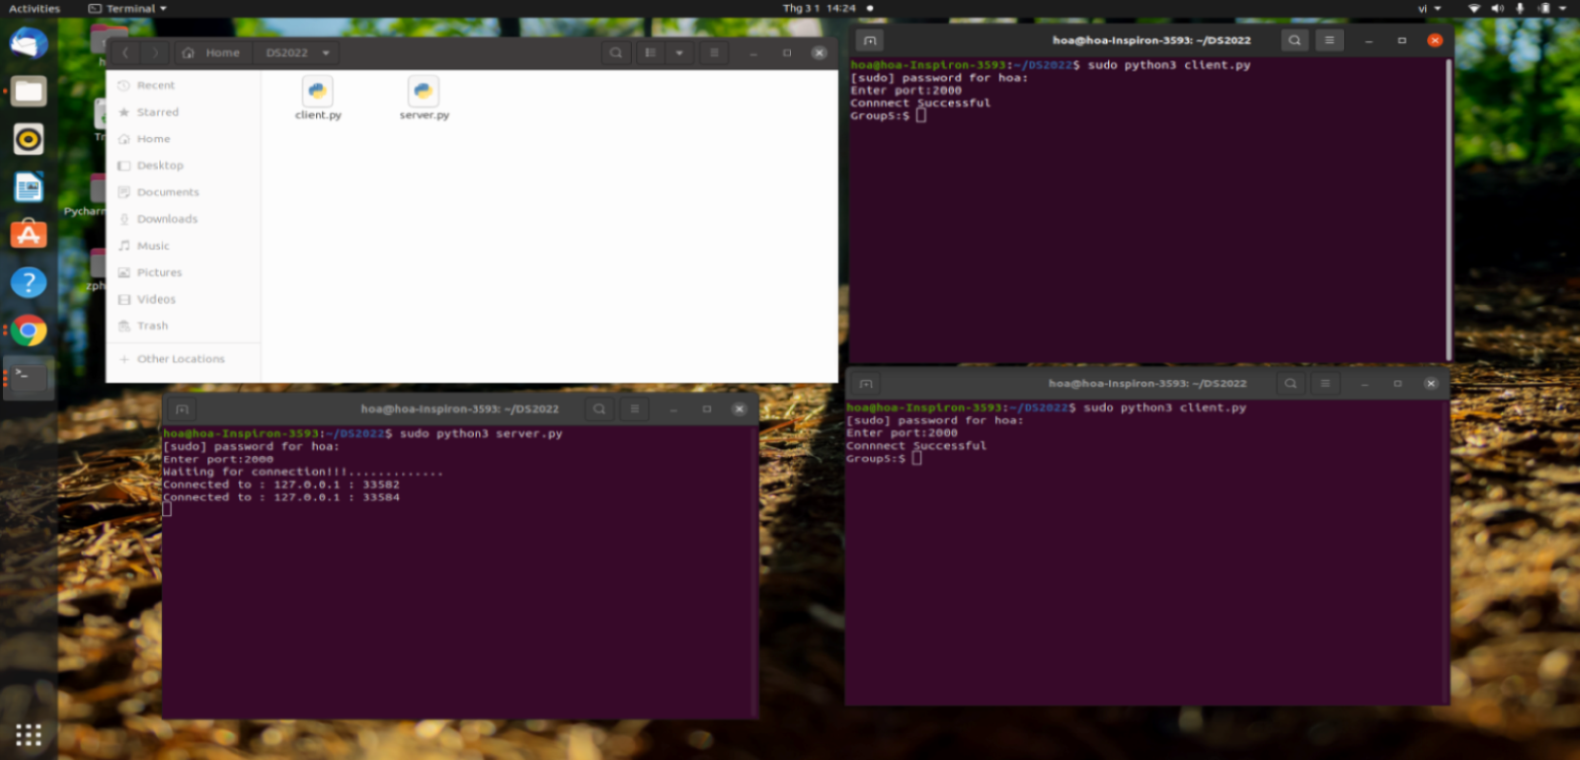
\includegraphics{images/result_3.png}
\end{figure}
\newpage
\hspace{0.7cm}Now that the connection is created, the client can execute any command line to the server. For example, client can create a folder named “test”:


\begin{figure}[h]
\centering
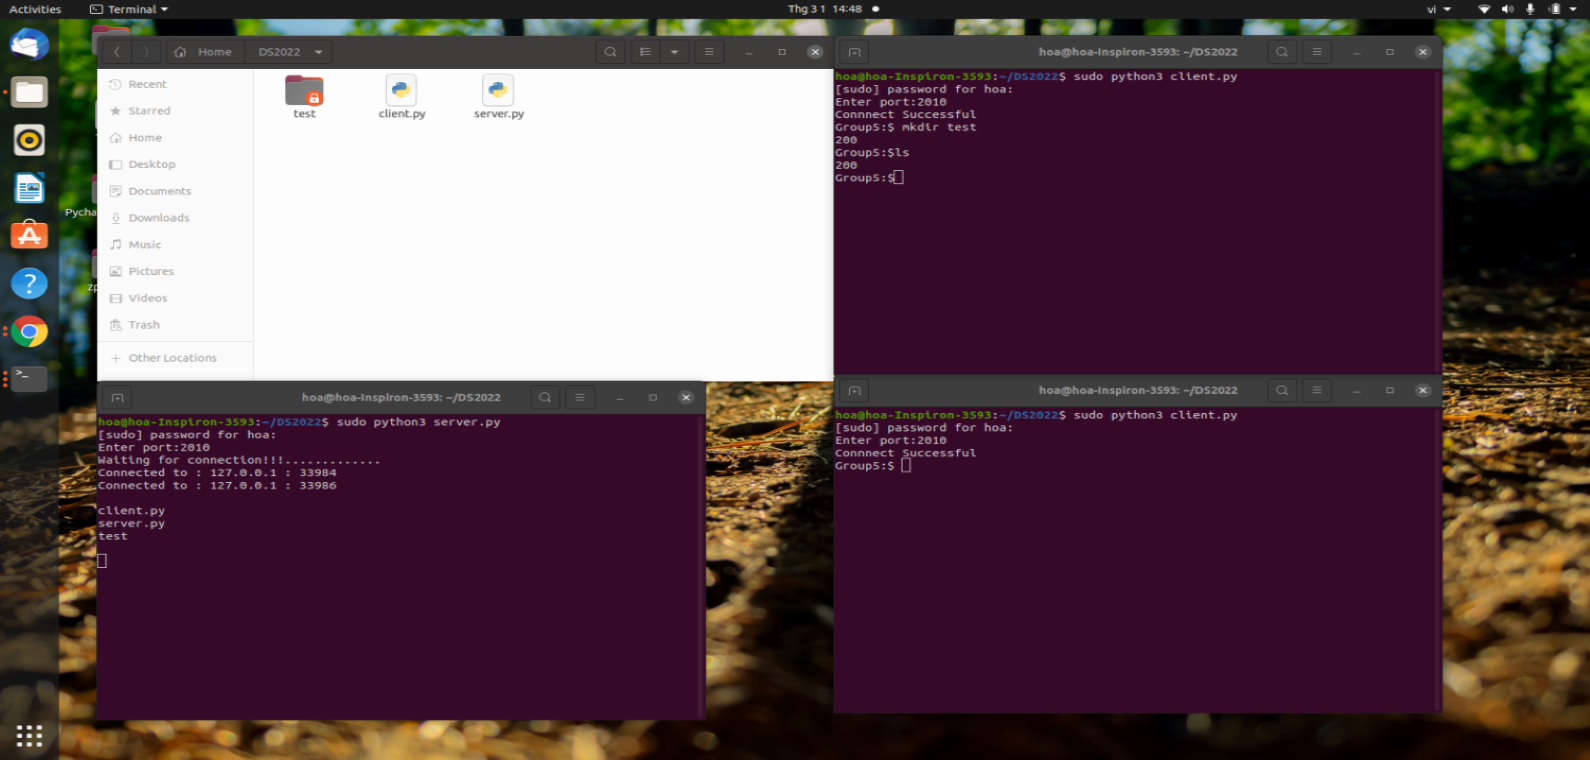
\includegraphics{images/result_4.png}
\end{figure}

\hspace{0.7cm}Then, client 1 wants to change path to that new folder and create a new text file named “text.txt”:

\begin{figure}[h]
\centering
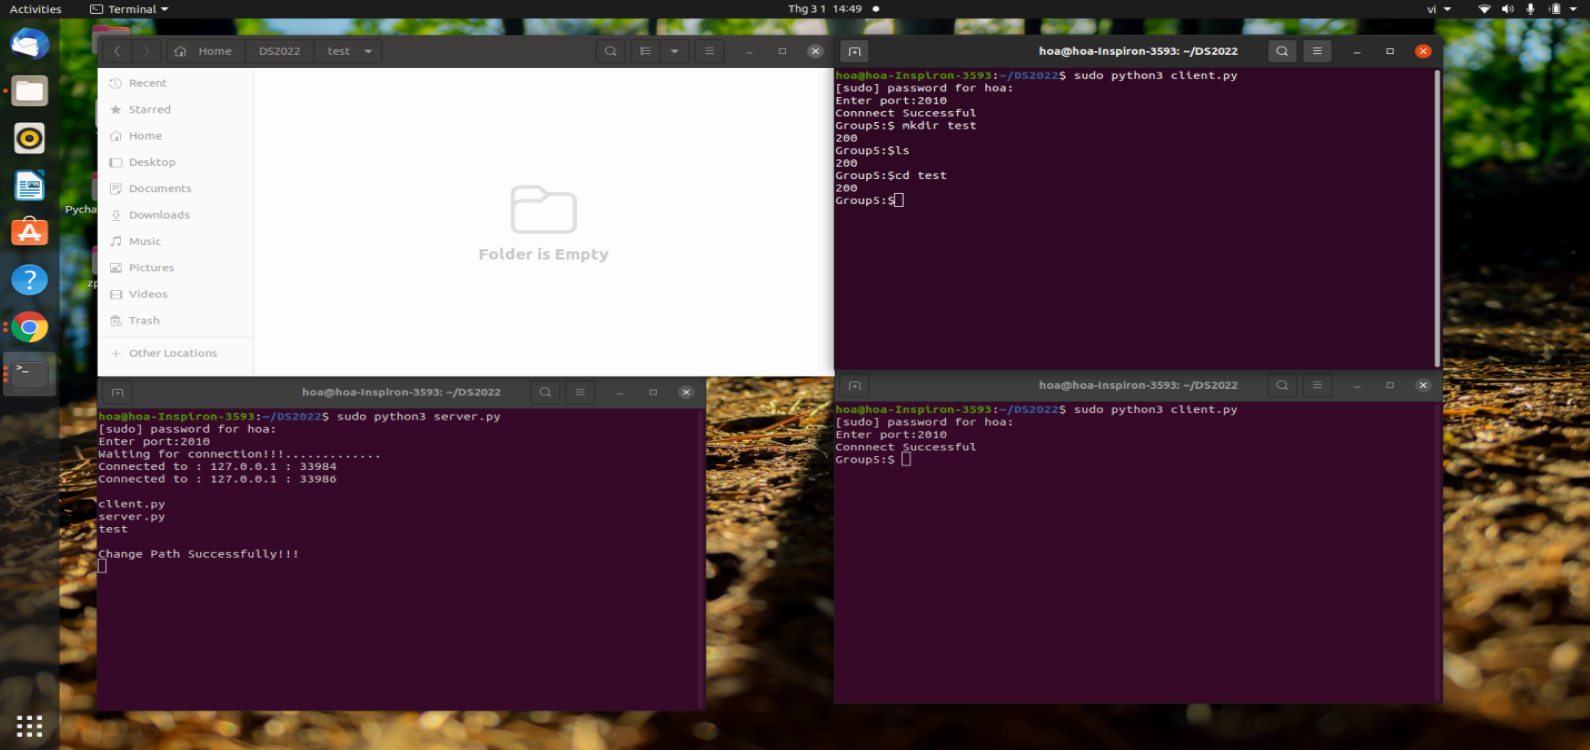
\includegraphics{images/result_5.png}
\end{figure}

\begin{figure}[h]
\centering
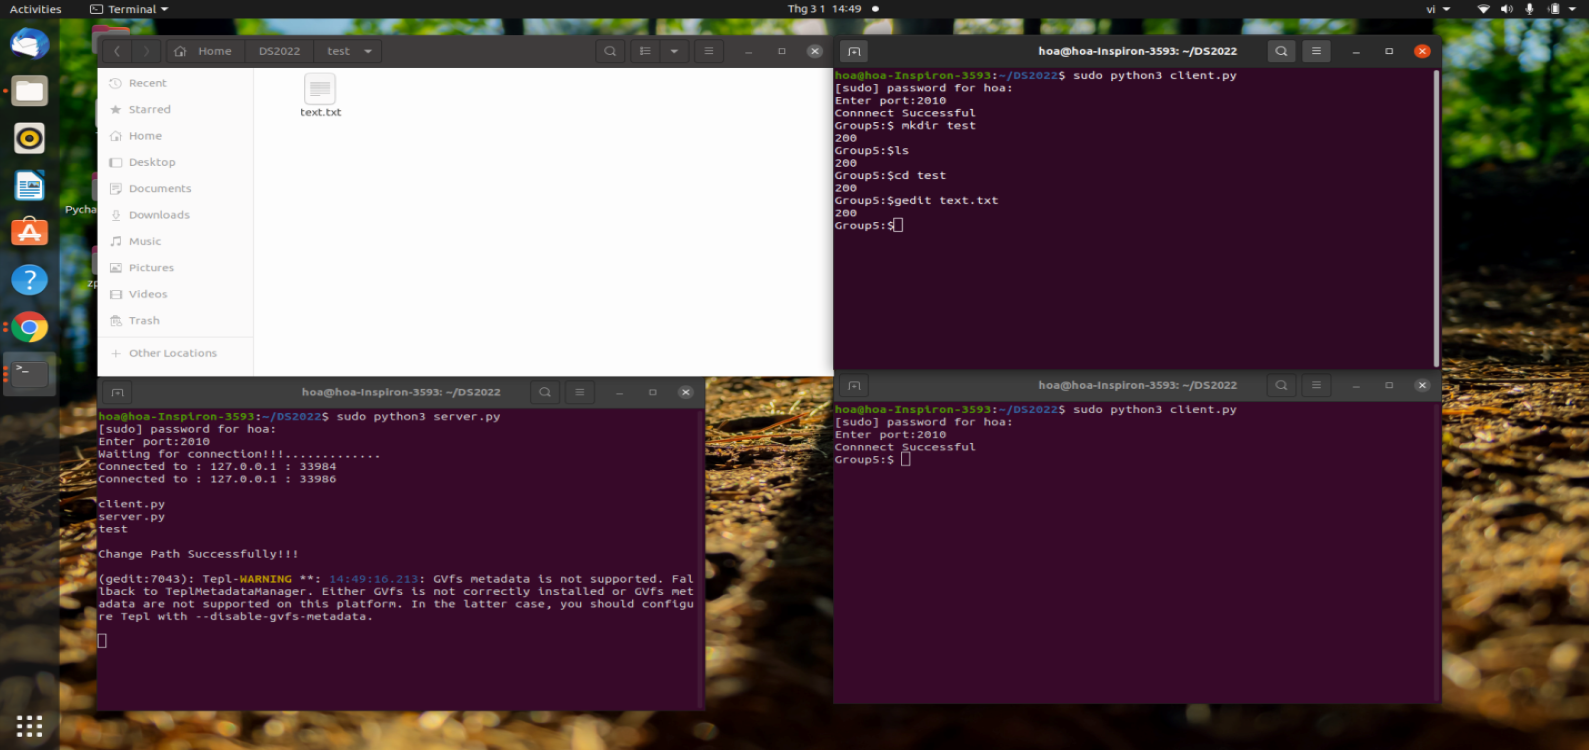
\includegraphics{images/result_6.png}
\end{figure}
\newpage

\hspace{0.7cm} Now, if client 2 want to delete the “text.txt” file that client 1 just created, he needs to change path to the “test” folder and delete the file:
\begin{figure}[h]
\centering
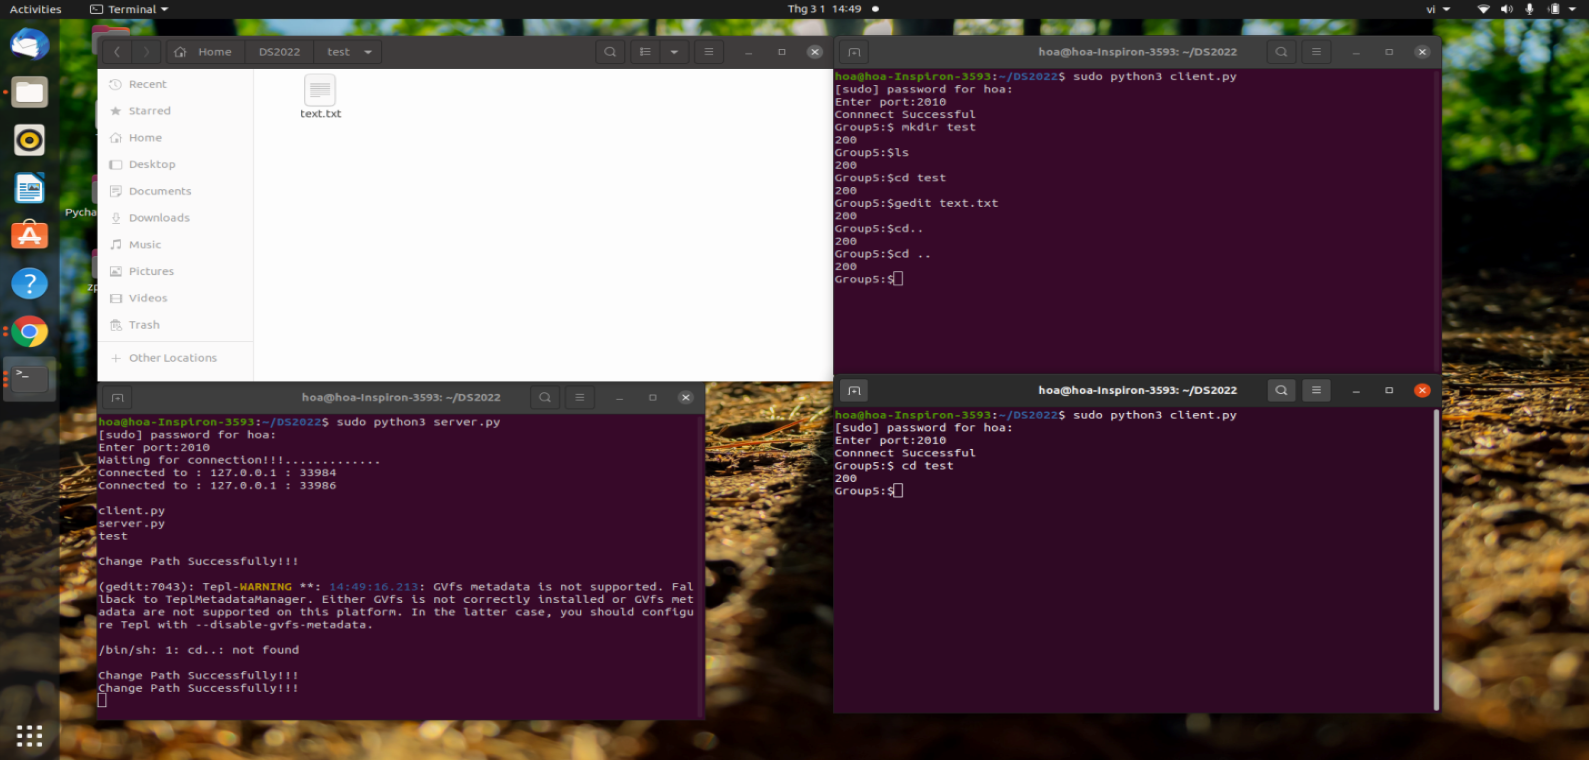
\includegraphics{images/result_7.png}
\end{figure}

\begin{figure}[h]
\centering
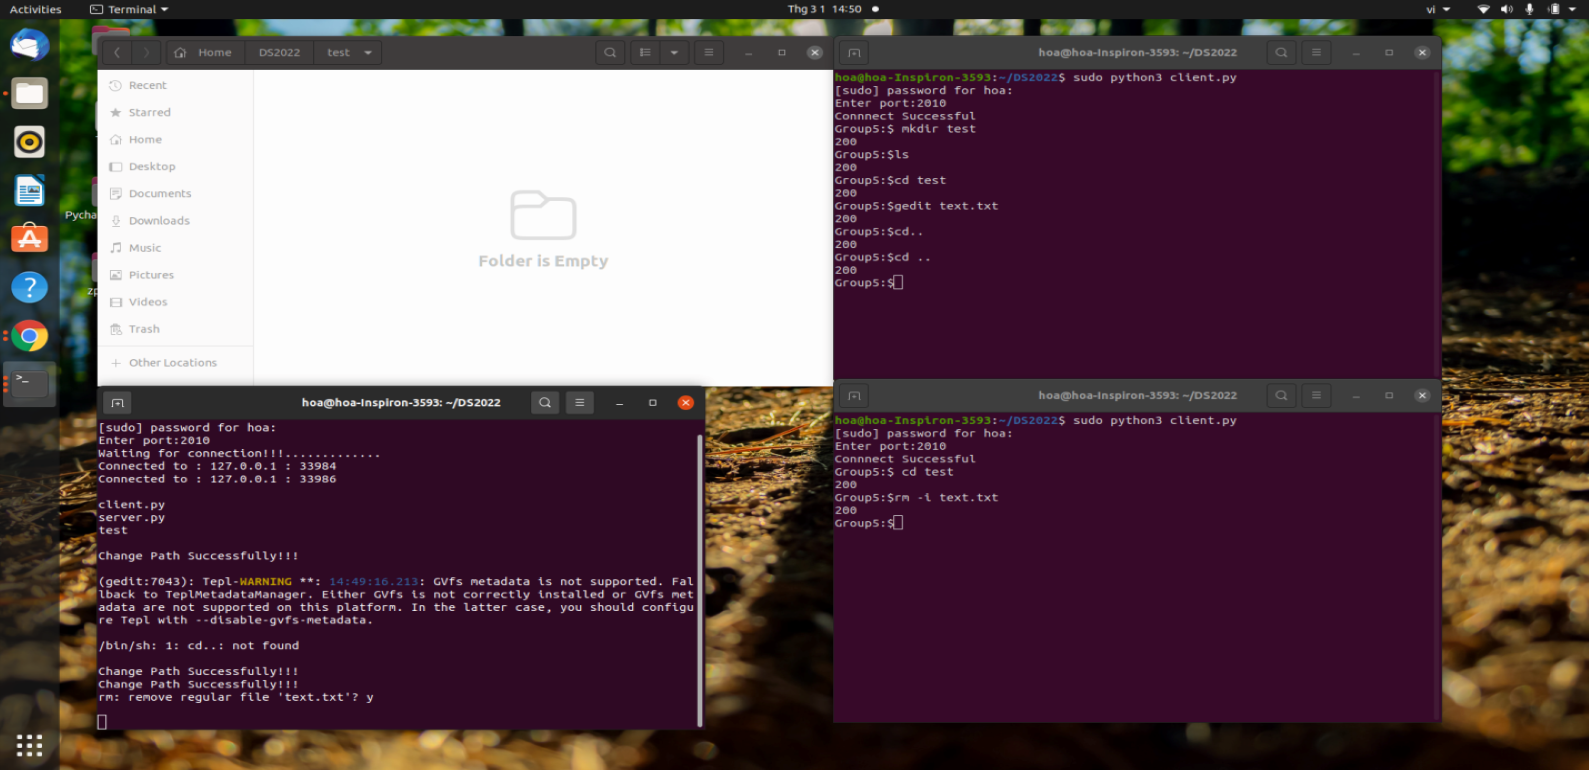
\includegraphics{images/result_8.png}
\end{figure}
\newpage
\hspace{0.7cm} Finally, if users want to end the working session, they must close the connection from the client side first to avoid the interference:

\begin{figure}[h]
\centering
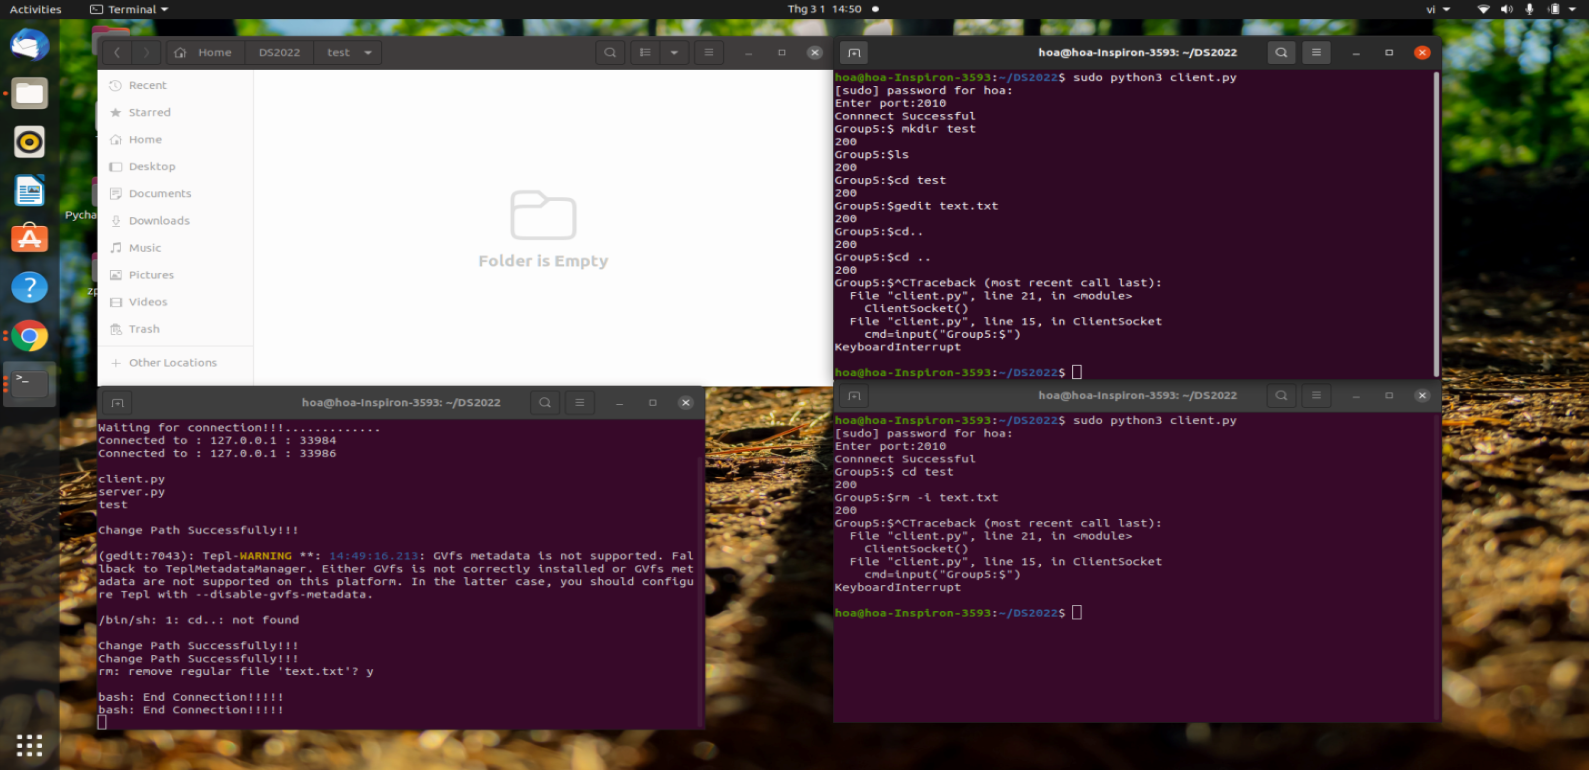
\includegraphics{images/result_9.png}
\end{figure}

\begin{figure}[h]
\centering
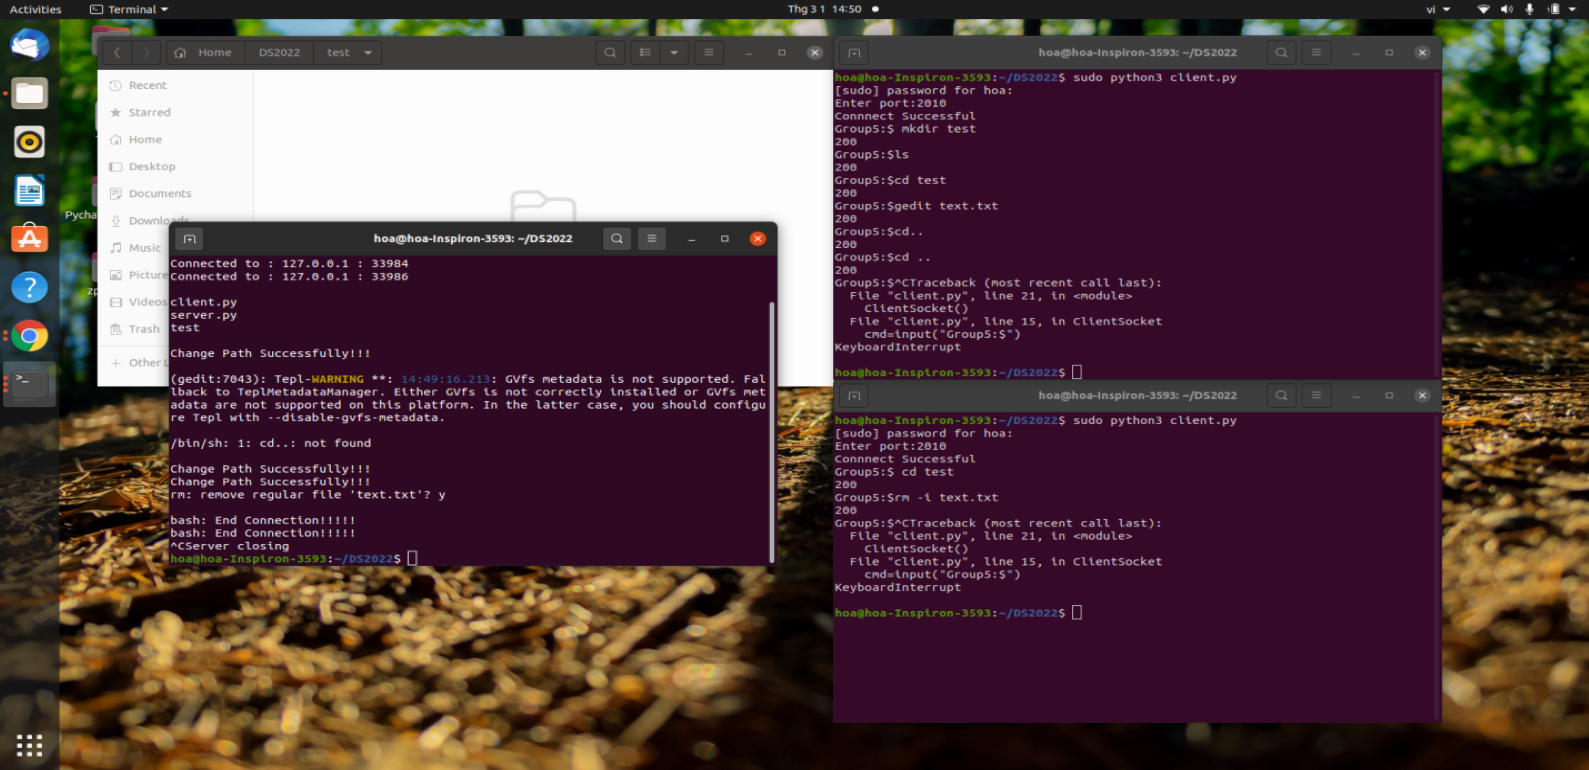
\includegraphics{images/result_10.png}
\end{figure}

\newpage
\hspace{0.7cm} 
